\chapter{Characteristics of Open Street Map}
	
\section{Introduction}
The OpenStreetMap is one of the most impressive projects of Volunteered Geographic Information on the Internet\cite{Neis2012}. Until recent the mapping of the Earth was preserved highly skilled, well-equipped and organized individuals and groups. One important happening was in 2000 when Bill Clinton removed the selective availability of the GPS signal \ref{sec:weber}. This change improved the accuracy of simpler, cheaper GPS receivers so that also ordinary people could start mapping their movements. OpenStreetMap was founded in 2004 at University College London by Steve Coast. The goal was to create a free database with geoxgraphic information of the world \cite{Neis2012}. Back in 2004 the geographic data was expencieve and hard to get access to. 

The OSM project stands out from other data sources mainly because its free to use and its released under a license that allows for pretty much whatever the user wants to as long as the user mention the original creator and the licence\cite{Chilton}.  The most common contribution approach is to record data using a GPS receiver and edit the data using one of the free and available OSM editors \cite{Neis2012}.  

Today the world has a need for instant information, particularly in crisis situations \cite{Chilton}. Here OpenStreetMap is the leading global example of the effictiveness of crowdsourcing of geodata. The project are changing the way individuals and organisations are thinking about the collection process, purchase and use of geodata \cite{Chilton}.  Crowd sourced geographic data has characteristics or advantages of large data volume, high currency, large quantity of information and low cost \cite{Wang2013}.  

\section{Culture}
OSMhas no notability rule, an arbitrary amount of detail is possible, but somebody has to maintain it! %https://www.youtube.com/watch?v=KNTSZGnQVRw

\section{Structure}
OpenStreetMap uses a topological data structure. This sturcture includes three basic components nodes, ways and relations. Nodes are points with a geographic position stored as coordinates (Lat, long) according to WGS84. Ways are lists of 2 or more nodes, representing a poly-line or polygon, used to represent streets, rivers, among others \cite{Debruyne2015}. A relation is a multi-purpose data structure that documents a relation between two or more components\href{https://wiki.openstreetmap.org/wiki/Elements}. To add metadata to geographic objects OpenStreetMap uses Tags. Tags consist of two items, a key and a value of the form key=value. The key is used to describe the topic, category or type of feature, while the value describes the details of the specific form of the key specified. A example of a key-value pair can be building=church, here the key is building and the value is church, this is a building that was built as a church. 

The norm in OSM is to try to map new data with existing tags. Good practice is to search for tags, or Map Features, on different OSM wiki-sites. On the \href{http://wiki.openstreetmap.org/wiki/Any_tags_you_like}{tags you like wikipage} they recommend different sites, but points out \href{http://taginfo.openstreetmap.org/}{taginfo} as the most useful site. Taginfo is a website created for finding and aggregating information about OSM tags, it covers the whole planet and is updated daily. The web page list tags used in the database and also inform on how often they have been used. Also, Taginfo lists other tags which have been used in combination with the tags you searched for. Some countries also have their own taginfo web pages, like Ireland, Great-Britain and France, Norway do not have their own taginfo web page. 

Verifiability: From a given scenario, a tag/value combination is verifiable if and only if independent users when observing the same feature would make the same observation every time.\href{http://wiki.openstreetmap.org/wiki/Verifiability}. 

\section{Organizational}
%Redgjøre for hva OSM er og hvordan det fungerer teknisk og organisatorisk
Organization and communication 

The OpenStreetMap Project is supported by the OpenStreeMap Foundation (OSMF) which is a UK-registered non-profit organization. The foundation was founded in 2006 and consists of members from all over the world, as of December 2015 consist of 350 normal-, 351 associate- and 18 corporate members \cite{OSMF2015}. OSMF include a board of seven members and is critical to the ongoing function and growth of the OpenStreetMap project \cite{OSMF}.  The foundation has the responsibility for the servers and services necessary for hosting the OSM project. Also, they support and communicates with the working groups, and delegates tasks that has to be done, like Web site development etc. 

A person can contribute to the OSM project without being a member of the foundation. The project has over 3 million registered users \cite{OSMProject2016} who are collecting and updating data. The crowdsourced data are then released under the Open Database License, \textit{"a license agreement intended to allow users to freely share, modify, and use this Database while maintaining this same freedom for others"} \cite{ODbL}.  Users can edit maps through different tools made by different OSM contributors. One tools is called iD and is the default web browser editor written by MapBox. There are also desktop editing applications like JOSM and Merkaartor which are more powerful and better suited for advanced users. 

Communication is country-mailing lists, wiki-pages and conferences. State of the map is the main OSM conference. Number of mappers and organizations are constantly increasing, what started as a crazy hacker project is now a vital part of the global data ecosystem. The community are constantly developing new ways to contribute.  Users can join a mapathon in their hometown, they can sit at home adding data, 

\href{http://2016.stateofthemap.org/2016/a-map-of-openstreetmap/}{The degree to how you can get involved in OSM is so deep, mapping, software processes etc. - keeps people interested. One problem is the communication through the different groups, the energy level is not high enough.  Lots of people exited about communication, everyone have a obligation to show the users their different possibilities}.   

Communication through mailing lists works for the people who subscribes to that list, but with over 150 different list it is impossible for an interested user to stay updated with all the latest achievements.  What is happening in the mailing lists has to be available to everyone in the community. A solution to this is called weeklyOSM. It started in 2010 in German, who alone has 50 different mailing lists. The weeklyOSM team are scanning mailing lists, twitter, blogs and so on. There are a international team translating the German blog into different languages. Little by little the rest of the community gets involved, translating the blog into languages thats not supported. 

There are different groups creating the different versions. The goal is to integrate more languages. There are a lot of work every week, hard to find volunteers. 

%Mer om OSM Foundation Success & Scale in a Data-Producing Organization s 4119, Org&ikt mappen

 \section{File format, .osm files}
The .osm file format is specific to OpenStreetMap and it is not easy to open these files using GIS-software like QGIS. The file format is designed to be easily sent and received across the internet in a standard format. Therefore .osm files are easily obtained, but using the files directly to do analysing and map design is not easy. The .osm files are coded in the XML format. It is recommended to convert the data into other formats when using the files \href{http://learnosm.org/en/osm-data/file-formats/}{source}. 

Points are represented as nodes, lines as ways and areas as relation in .osm files. Each represented by a tag: <node>, <way> and <relation>. Node is one of the core elements in the OSM data model. A node-tag consists of a single point defined by node-id, latitude and longitude. When nodes are used on their own they represents point features, normally includes at least one tag to define the points purpose \cite{OpenStreetMapc}. In figure \ref{fig:nodetag} the node tag represents a bag shop named Citybag, a point of interest, where k is key and v is value. User is the name of who last modified the node and uid is the persons numeric user id.  

\begin{figure}[H]
    \centering
    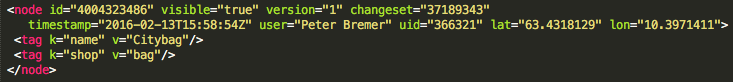
\includegraphics[scale=0.6]{figures/FixedByMe/node_tag.png}
    \caption{Example of a node tag}
    \label{fig:nodetag}
\end{figure} 

A way consists of two or more nodes and can either be open or closed. An open way describes a line feature not sharing first and last node. Features can be roads, cycleway, streams etc.* %Kan man skrive etc paa engelsk?
When a way is closed the first and last nodes are the same and can be interpreted as a closed polyline or an area, or both \cite{OpenStreetMapd}. A closed way with highway=* tag can represent roundabouts, and if it has amenity=school tag the closed way can represent the outline of a school. In figure \ref{fig:waytag} the way represents a building since k=building and v=yes. The buildings address is also added and its name. The <nd> tag represents a node, where all the <nd> tags creates the building footprint. Note that the first and last <nd> tag refers to the same node. 

\begin{figure}[H]
    \centering
    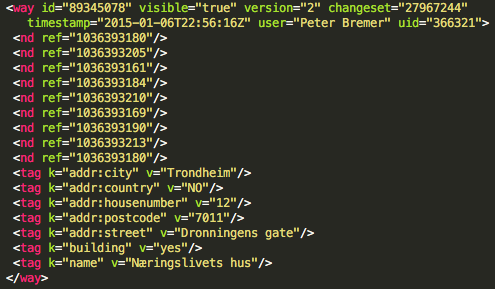
\includegraphics[scale=0.7]{figures/FixedByMe/way_tag.png}
    \caption{Example of a way tag}
    \label{fig:waytag}
\end{figure} 

A relation is an ordered list of one or more nodes, ways and/or relations. 



 
